%
% $RCSfile: architecture.tex,v $
%
% Copyright (C) 2002-2008. Christian Heller.
%
% Permission is granted to copy, distribute and/or modify this document
% under the terms of the GNU Free Documentation License, Version 1.1 or
% any later version published by the Free Software Foundation; with no
% Invariant Sections, with no Front-Cover Texts and with no Back-Cover
% Texts. A copy of the license is included in the section entitled
% "GNU Free Documentation License".
%
% http://www.cybop.net
% - Cybernetics Oriented Programming -
%
% http://www.resmedicinae.org
% - Information in Medicine -
%
% Version: $Revision: 1.1 $ $Date: 2008-08-19 20:41:05 $ $Author: christian $
% Authors: Christian Heller <christian.heller@tuxtax.de>
%

\section{Architecture}
\label{architecture_heading}
\index{CYBOI Architecture}

The following sections dwell on how CYBOI fits into a general computer
architecture, and then explain its inner structure and software patterns used.

%
% $RCSfile$
%
% Copyright (c) 2005-2006. Christian Heller. All rights reserved.
%
% Permission is granted to copy, distribute and/or modify this document
% under the terms of the GNU Free Documentation License, Version 1.1 or
% any later version published by the Free Software Foundation; with no
% Invariant Sections, with no Front-Cover Texts and with no Back-Cover
% Texts. A copy of the license is included in the section entitled
% "GNU Free Documentation License".
%
% http://www.cybop.net
% - Cybernetics Oriented Programming -
%
% http://www.resmedicinae.org
% - Information in Medicine -
%
% Version: $Revision$ $Date$ $Author$
% Authors: Christian Heller <christian.heller@tuxtax.de>
%

\subsubsection{Overall Placement}
\label{overall_placement_heading}

Considering an overall computer system architecture, \emph{CYBOI} is situated
between the application knowledge existing in form of \emph{CYBOL} templates
and the \emph{Hardware} controlled by an \emph{Operating System} (OS) (figure
\ref{connection_figure}). CYBOI can thus also be called a
\emph{Knowledge-Hardware-Interface} (synonymous with \emph{Mind-Brain-Interface}).

\begin{figure}[ht]
    \begin{center}
        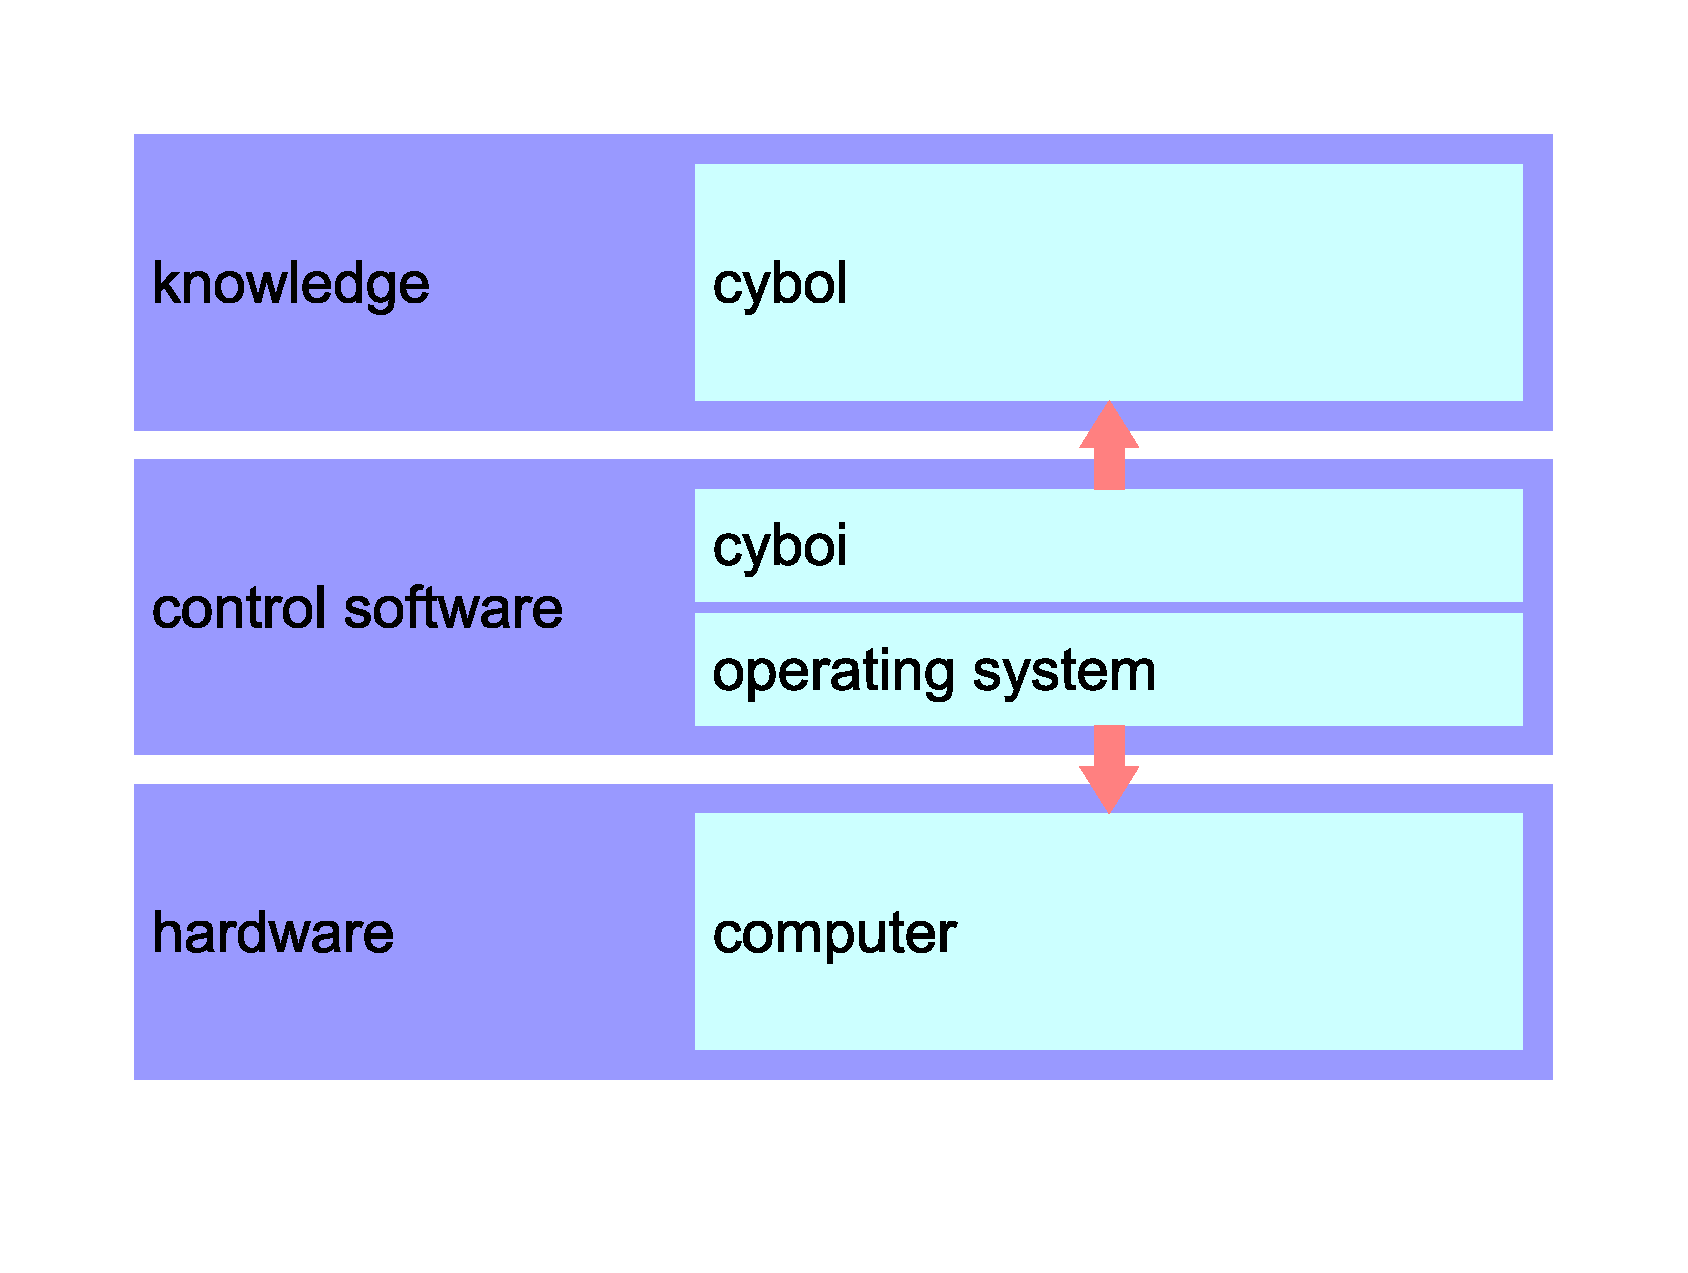
\includegraphics[scale=0.2]{vector/connection.eps}
        \caption{Knowledge -- Hardware Link}
        \label{connection_figure}
    \end{center}
\end{figure}

\begin{table}[ht]
    \begin{center}
        \begin{footnotesize}
        \begin{tabular}{| p{18mm} | p{18mm} | p{18mm} |}
            \hline
            \textbf{Criterion} & \textbf{Java World} & \textbf{CYBOP World}\\
            \hline
            Theory & OOP in Java & CYBOP\\
            \hline
            Language & Java & CYBOL\\
            \hline
            Interpreter & Java VM & CYBOI\\
            \hline
        \end{tabular}
        \end{footnotesize}
        \caption{Java-/ CYBOP World Analogies}
        \label{analogies_table}
    \end{center}
\end{table}

There are analogies to other systems run by language interpretation. Table
\ref{analogies_table} shows those between the \emph{Java-} and \emph{CYBOP}
world. Both are based on a programming theory, have a language and interpreter.
A theoretical model of a computer hardware- or -software system may be called
an \emph{Abstract Computer} or \emph{Abstract Machine} \cite{wikipedia}. If
being implemented as software simulation, or if containing an interpreter, it
is called a \emph{Virtual Machine} (VM). Kernighan and Pike write in their book
\emph{Practice of Programming} \cite{kernighan1999}:

\begin{quote}
� � Virtual machines are a wonderful, old idea, that latterly, through Java and
    the \emph{Java Virtual Machine} (JVM), came into fashion again. They are a
    simple possibility to gain portable and efficient program code, which can
    be written in a higher programming language.
\end{quote}

In that sense, CYBOI is certainly a VM. It provides low-level, platform-dependent
system functionality, close to the OS, together with a unified knowledge schema
(section \ref{knowledge_schema_heading}) which allows CYBOL applications to be
truly portable, well extensible and easier to program, because developers need
to concentrate on domain knowledge only. Since CYBOI interprets CYBOL sources
\emph{live} at system runtime, without the need for previous compilation (as in
Java), changes to CYBOL sources get into effect right away, without restarting
the system.

%
% $RCSfile: inner_structure.tex,v $
%
% Copyright (C) 2002-2008. Christian Heller.
%
% Permission is granted to copy, distribute and/or modify this document
% under the terms of the GNU Free Documentation License, Version 1.1 or
% any later version published by the Free Software Foundation; with no
% Invariant Sections, with no Front-Cover Texts and with no Back-Cover
% Texts. A copy of the license is included in the section entitled
% "GNU Free Documentation License".
%
% http://www.cybop.net
% - Cybernetics Oriented Programming -
%
% http://www.resmedicinae.org
% - Information in Medicine -
%
% Version: $Revision: 1.1 $ $Date: 2008-08-19 20:41:07 $ $Author: christian $
% Authors: Christian Heller <christian.heller@tuxtax.de>
%

\subsection{Inner Structure}
\label{inner_structure_heading}
\index{CYBOI Knowledge Container}
\index{CYBOI Signal Checker}
\index{Neumann Model of a Computing Machine}

To what concerns its inner architecture, there are two basic structures
underlying CYBOI:

\begin{enumerate}
    \item \emph{Knowledge Container:} An array-based structure usable for
        storing static knowledge in form of primitive- and compound models, and
        capable of representing a map, collection, list and tree
    \item \emph{Signal Checker:} A loop-based structure usable for dynamically
        reading signals from a queue, and capable of processing them after
        their priority, in a special handler
\end{enumerate}

All modules, into which CYBOI is subdivided, are built around these two core
structures. Having read chapter \ref{state_and_logic_heading} demonstrating the
existence of state- and logic knowledge, one might argue that there should be
two knowledge containers, one for each kind. But because knowledge models may
be placed not only in space or time, but possibly other dimensions, too (like
mass, for the weights in an artificial neural network), the prototype emerging
from this work stores state- and logic-, as well as any other models in one and
the same knowledge tree.

Not unlike John von Neumann's model of a computing machine \cite{selflinux},
which distinguishes \emph{Memory}, \emph{Control Unit},
\emph{Arithmetic Logic Unit} (ALU) and \emph{Input/ Output} (i/o), CYBOI's
modules are grouped into four architectural parts, as illustrated in figure
\ref{architecture_figure}. These have the following functionality:

\begin{itemize}
    \item \emph{Memoriser:} data creation, -destruction and -access (after
        Neumann, it contains not only data, but also the operations that are
        applied to them)
    \item \emph{Controller:} lifecycle management, signal handling, i/o filters
    \item \emph{Applicator:} operation application (comparison, logic,
        arithmetic and more)
    \item \emph{Globals:} basic constants and variables, as well as a logger
\end{itemize}

\begin{figure}[ht]
    \begin{center}
        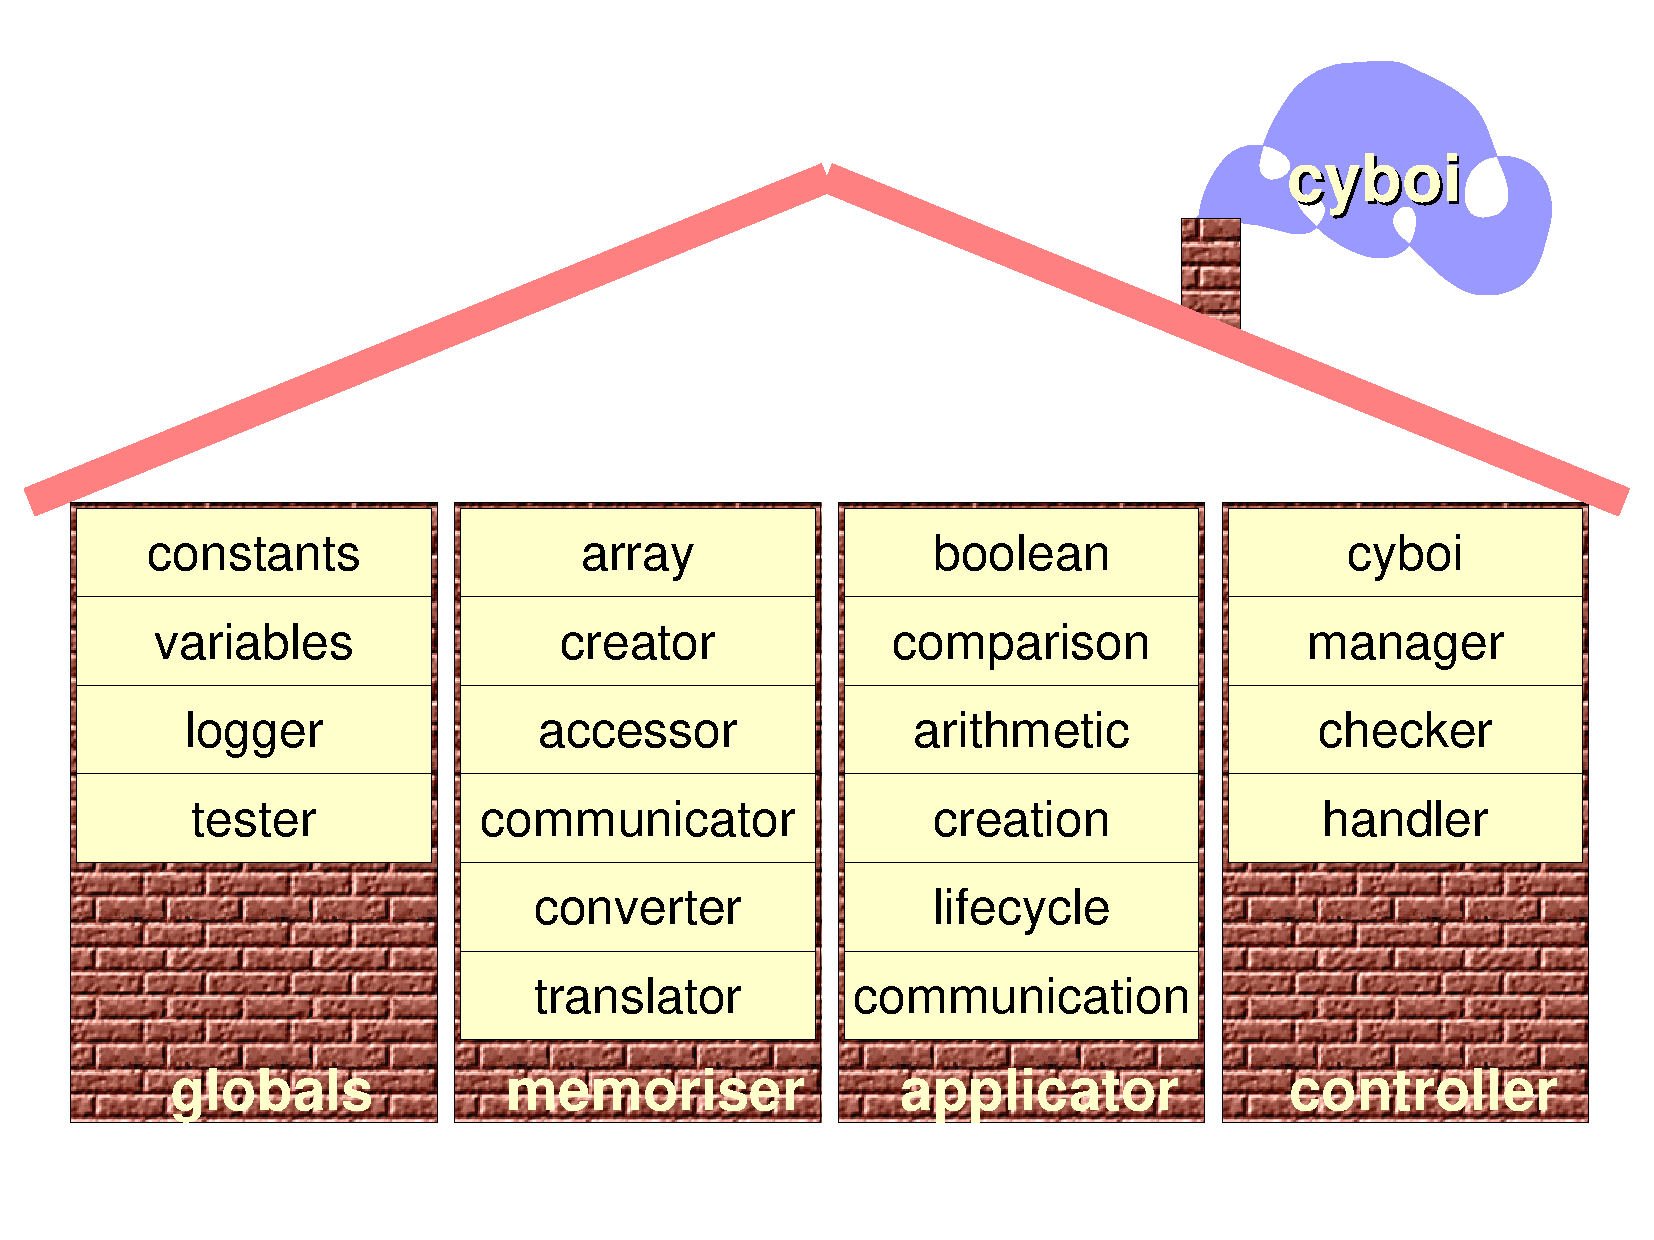
\includegraphics[scale=0.3,angle=-90]{graphic/architecture.pdf}
        \caption{CYBOI Architecture consisting of Four Parts}
        \label{architecture_figure}
    \end{center}
\end{figure}

The i/o data handling is not separated out here (as opposed to von Neumann's
model); it is managed by the controller modules. The i/o data themselves,
representing states, are stored in memory. Global constants and variables are
necessary additions. More details on the modules' functionality are given in
section \ref{functionality_in_detail_heading}.

%
% $RCSfile: pattern_merger.tex,v $
%
% Copyright (C) 2002-2008. Christian Heller.
%
% Permission is granted to copy, distribute and/or modify this document
% under the terms of the GNU Free Documentation License, Version 1.1 or
% any later version published by the Free Software Foundation; with no
% Invariant Sections, with no Front-Cover Texts and with no Back-Cover
% Texts. A copy of the license is included in the section entitled
% "GNU Free Documentation License".
%
% http://www.cybop.net
% - Cybernetics Oriented Programming -
%
% http://www.resmedicinae.org
% - Information in Medicine -
%
% Version: $Revision: 1.1 $ $Date: 2008-08-19 20:41:08 $ $Author: christian $
% Authors: Christian Heller <christian.heller@tuxtax.de>
%

\subsection{Pattern Merger}
\label{pattern_merger_heading}
\index{CYBOI using Patterns}
\index{Model View Controller Pattern in CYBOI}
\index{MVC in CYBOI}
\index{Data Mapper Pattern in CYBOI}
\index{Data Transfer Object Pattern in CYBOI}
\index{DTO in CYBOI}
\index{Pipes and Filters Pattern in CYBOI}
\index{Microkernel Pattern in CYBOI}
\index{Broker Pattern in CYBOI}
\index{CYBOI as Peer to Peer System}
\index{CYBOI as GUI Renderer}
\index{Pattern-less Application Development in CYBOI}

A variety of software patterns (section \ref{pattern_heading}) can be found
when inspecting CYBOI's architecture. Most of them, especially those relying on
\emph{Object Oriented} (OO) principles, are used in an \emph{adapted} form, as
described following.

Firstly, there are those that can be summed up under the umbrella term
\emph{Translator Patterns}: \emph{Model View Controller} (MVC),
\emph{Data Mapper} and \emph{Data Transfer Object} (DTO). As section
\ref{translator_architecture_heading} tried to show, they all contain two state
models, one logic model and a controlling unit, which is why it is possible to
unify- and place them into one common architecture. CYBOI represents the unit
controlling all action, on a low system level. It stores state- as well as
logic models in one common knowledge tree, and uses the rules encoded in logic
models to translate state models into each other.

Secondly, there is the \emph{Pipes and Filters} pattern which CYBOI uses not
only to instantiate knowledge templates, but also for system communication.
An input (i/p) state (like a persistent, serialised knowledge template) runs
through a cascade of filters, namely \emph{Creator}, \emph{Communicator},
\emph{Converter} and \emph{Translator}, before it is processed (as transient
knowledge model) inside the system, to be finally forwarded in opposite
direction through the same filters, resulting in an output (o/p) state.

Thirdly, CYBOI acts as \emph{Microkernel} and \emph{Broker}, at the same time.
It calls special threads (internal servers) managing data input/ output (i/o),
and has the capability to communicate with remote systems (external servers),
for data transfer. The actual impulse for communication comes from a passive
knowledge model (adapter) that is actively processed by CYBOI. Since that
impulse is \emph{not} a direct method call, but either a \emph{send-} or
\emph{receive} operation with varying parameters, special \emph{Proxy} models
are not needed anymore. CYBOI may act as client and server, at the same time,
which enables the applications running within it to act as \emph{Peer to Peer}
(P2P) systems (section \ref{peer_node_heading}). It incorporates a signal
(event) loop (like the broker) and handles low-level system (socket)
communication (like the bridge).

The fact that future versions of CYBOI will be able to interpret CYBOL
knowledge templates containing \emph{Graphical User Interface} (GUI)
descriptions, makes it a \emph{GUI Renderer}. The task of a renderer is to
translate GUI models into hardware-understandable function calls and protocols.
%(section \ref{user_interface_modelling_heading}).
In the case of CYBOI, the
graphical environment supported first will be the \emph{X Window System} (X)
\emph{XFree86} \cite{xfree86} variant. The step towards rendering models given
in \emph{Hyper Text Markup Language} (HTML) format is not far then, so that
CYBOI may act not only as web server, but also as web browser. All that,
together with further additions, will make it virtually an \emph{All-Rounder}
system.

The usage of simplified forms of patterns like \emph{Composite} (inheritance
omitted), \emph{Whole-Part}, \emph{Wrapper} or \emph{Layers}, for knowledge
storage, was already mentioned in section \ref{hidden_patterns_heading}.

Unfavourable patterns as mentioned in section \ref{pattern_systematics_heading}
(those with \emph{global access} or \emph{bidirectional dependencies}) were
avoided.

Finally, the merged appearance of patterns in CYBOI (and CYBOL for that matter)
brings software development one step closer to \emph{pattern-less} application
programming. Application developers are freed from the burden of repeatedly
figuring out suitable patterns, and enabled to concentrate on modelling pure
domain knowledge, based on the concept of \emph{Hierarchy}, instead.

%
% $RCSfile: kernel_concepts.tex,v $
%
% Copyright (C) 2002-2008. Christian Heller.
%
% Permission is granted to copy, distribute and/or modify this document
% under the terms of the GNU Free Documentation License, Version 1.1 or
% any later version published by the Free Software Foundation; with no
% Invariant Sections, with no Front-Cover Texts and with no Back-Cover
% Texts. A copy of the license is included in the section entitled
% "GNU Free Documentation License".
%
% http://www.cybop.net
% - Cybernetics Oriented Programming -
%
% http://www.resmedicinae.org
% - Information in Medicine -
%
% Version: $Revision: 1.1 $ $Date: 2008-08-19 20:41:07 $ $Author: christian $
% Authors: Christian Heller <christian.heller@tuxtax.de>
%

\subsection{Kernel Concepts}
\label{kernel_concepts_heading}
\index{Operating System Concepts in CYBOI}
\index{OS Concepts in CYBOI}
\index{Kernel Concepts in CYBOI}
\index{CYBOI as Monolithic Kernel}
\index{CYBOI as Microkernel}
\index{CYBOI as Hybrid Kernel}
\index{CYBOI as Exokernel}
\index{CYBOI as Hardware Abstraction Layer}
\index{CYBOI avoiding Inter Process Communication}

Although certainly not qualifying as \emph{Operating System} (OS), CYBOI uses
some similar concepts. However, it is not easy to assign CYBOI to one of the four
broad categories of OS kernels, which the Wikipedia Encyclopedia \cite{wikipedia}
describes as follows:

\begin{enumerate}
    \item \emph{Monolithic Kernels:} providing rich and powerful abstractions
        of the underlying hardware
    \item \emph{Microkernels:} providing a small set of simple hardware abstractions
        and using applications called servers to provide more functionality
    \item \emph{Hybrid Kernels:} being much like pure microkernels, except that
        they include some additional code in kernelspace to increase performance
    \item \emph{Exokernels:} providing minimal abstractions but allowing the
        use of library operating sytems to provide more functionality via
        direct or nearly direct access to hardware
\end{enumerate}

Just like a \emph{Monolithic Kernel}, CYBOI encapsulates low-level functionality
like memory management and provides a high-level virtual interface (operations),
over which CYBOL applications may access it. Although the processing of signals
happens in its main process, CYBOI has to rely on a few communication services,
running in their own threads, and control their data exchange. This is (roughly)
comparable to the \emph{Microkernel} design which was mentioned as pattern in
section \ref{pattern_merger_heading} before. But these services sharing a common
address space (\emph{Internals Memory} and \emph{Signal Memory}) with the CYBOI
kernel, actually makes CYBOI a \emph{Hybrid Kernel}. The only existing data in
user address space (\emph{Knowledge Memory}) are knowledge models that have been
created from CYBOL knowledge templates. The kernel category coming closest to
CYBOI's design, however, is the \emph{Exokernel}. This is because CYBOI, though
serving as \emph{Hardware Abstraction Layer} (HAL) to CYBOL applications (what
is actually known from classic monolithic- and microkernels), also has a central
\emph{Signal Checker} control loop calling subroutines managing a part of the
hardware or software, which, after \cite{wikipedia}, were one of the simplest
methods of creating an exokernel.

The above-mentioned services provide \emph{Input/ Output} (i/o) functionality
to CYBOI so that it can communicate (\emph{virtual world}) ideas with other
(human or technical) systems, across (\emph{real world}) hardware. The services
may be configured, started up, interrupted and shutdown via CYBOL operations.
Similar to the \emph{Self Awareness} of human systems (mentioned in section
\ref{self_awareness_heading}), a CYBOL application has to know about available
i/o services, in order to actually use them. This configuration information may
be stored in CYBOL files as well.

Another thought turns around the \emph{Process} concept \cite{tanenbaum2001},
which is used to share computing time of the \emph{Central Processing Unit}
(CPU) as well as resource space in \emph{Random Access Memory} (RAM) between
applications. One then says: \textit{Every application runs in a separate
process.} The example environment in chapter \ref{physical_architecture_heading}
contained many different kinds of inter-communicating systems, not all of which
have to run on a separate physical machine, but surely in a separate process,
if on one-and-the-same machine. That way, one machine may host multiple
application systems.

However, the existence of many program processes running concurrently in an OS
holds conflicts. It necessitates ways for \emph{Inter-Process Communication}
(IPC), that assure the integrity of data in memory and avoid deadlocks
(blocking of the system). Common IPC methods include \cite{ipc, tanenbaum2001}:
\emph{Pipes} and \emph{Named Pipes}, \emph{Message Queueing}, \emph{Semaphores},
\emph{Shared Memory} and \emph{Sockets}.

A different approach was chosen in CYBOI: It is the only process running. CYBOL
applications reside as separate knowledge models in the \emph{Knowledge Memory}
(user address space), and CYBOI controls them all. This is the exact opposite
of running one process per application. However, it is unclear, at first, how
multiple applications running in parallel receive their corresponding signals.
CYBOI needs to evaluate incoming signals and then call the right logic of the
right application. But how to do that?

The application to which a signal is sent can be identified, depending on the
communication mechanism used. A \emph{keyboard\_pressed} or \emph{mouse\_clicked}
event, for example, always references the top-most window in a GUI environment.
Menu-, toolbar- and other buttons of the top-most window in turn reference a
logic (algorithm) whose dot-separated name starts with that of the application.
Within CYBOI, applications have to have a unique name, of course, so that
signals can be addressed correctly, to the right receiver. Once a logic routine
is identified, it can be sent as new signal to be processed by the signal loop.
Another example would be signals arriving over network. Also here, applications
can be identified, for example by a special \emph{Port} that was assigned to
them beforehand. A remote call references a specific logic by name so that it
can be processed locally. Equally named local procedures are distinguished by
the application name identified before. Within an application, logic names have
to be unique, of course.

%
% $RCSfile: security.tex,v $
%
% Copyright (C) 2002-2008. Christian Heller.
%
% Permission is granted to copy, distribute and/or modify this document
% under the terms of the GNU Free Documentation License, Version 1.1 or
% any later version published by the Free Software Foundation; with no
% Invariant Sections, with no Front-Cover Texts and with no Back-Cover
% Texts. A copy of the license is included in the section entitled
% "GNU Free Documentation License".
%
% http://www.cybop.net
% - Cybernetics Oriented Programming -
%
% http://www.resmedicinae.org
% - Information in Medicine -
%
% Version: $Revision: 1.1 $ $Date: 2008-08-19 20:41:08 $ $Author: christian $
% Authors: Christian Heller <christian.heller@tuxtax.de>
%

\subsection{Security}
\label{security_heading}
\index{Security in CYBOI}
\index{CYBOI as Secure Architecture}
\index{CYBOI as Capability Based System}
\index{CYBOI avoiding Access Control Lists}
\index{Capability Based System}
\index{Access Control List}
\index{ACL}
\index{Orthogonally Persistent Operating System}
\index{Flex Machine}
\index{Ten15}

Berin Loritsch of the former Apache Avalon Project \cite{avalon} writes that
system \emph{Security} has three distinct concerns, of which \emph{Encryption}
is only a part:

\begin{enumerate}
    \item \emph{Authentication:} authoritative validation of the identity of a
        party, such as a software component
    \item \emph{Authorisation:} deciding what access a component has to system
        resources
    \item \emph{Architecture:} usage of a proper, secure architecture
\end{enumerate}

Since this chapter is about CYBOI's architecture, what interests the most here
is point number three. But how to ensure a secure architecture? The avoidance
of global data access and bidirectional dependencies is clearly a requirement
(section \ref{recommendation_heading}), which CYBOI accomplishes through
disregard of the corresponding patterns (section \ref{pattern_merger_heading}).
Any kind of application knowledge resides in its \emph{Knowledge Memory}, whose
tree structure may be navigated along well-defined, unidirectional paths.

One may wonder how address spaces of the different applications are protected,
so that one application may not access another one's models? Traditionally, the
process concept assures that separation, but with CYBOI being the only process,
and all applications being part of it, another solution needs to be applied.
The exact mechanism to solve this in CYBOI yet has to be determined. However,
since all signals have to pass the same, central signal loop, they all can be
checked for permissions, before being processed, or filtered out, if necessary.
It would be imaginable and not difficult, to attach an application name as a
signal's origin, or a unique passphrase as additional meta information to a
signal memory's signals, that own an \emph{Identifier} (ID) anyway. The signal
loop or signal handler could then decide whether or not to send a signal to a
specific application.

Attached meta information of that kind would be comparable to a concept called
\emph{Capability}, which is known from \emph{Secure Computing}, a subfield of
\emph{Security Engineering} \cite{wikipedia}. It is the alternative to
\emph{Access Control Lists} (ACL), another means of enforcing firstly:
\emph{Mandatory Access Control}, and secondly: \emph{Privilege Separation}
(where an entity has only the privileges that are needed for its function).
Wikipedia \cite{wikipedia} writes on this:

\begin{quote}
    \emph{Capabilities} (also known as \emph{Key}) achieve their objective of
    improving system security by being used in place of \emph{Plain References}.
    A plain reference (for example, a path name) uniquely identifies an object,
    but does not specify which \emph{Access Rights} are appropriate for that
    object and the user program which holds that reference. Consequently, any
    attempt to access the referenced object must be validated by the operating
    system, typically via the use of an \emph{Access Control List} (ACL). In
    contrast, in a pure capability-based system, the mere fact that a user
    program possesses that capability entitles it to use the referenced object
    in accordance with the rights that are specified by that capability. In
    theory, a pure capability-based system removes the need for any ACL or
    similar mechanism, by giving all entities all and only the capabilities
    they will actually need.
\end{quote}

With almost all important \emph{Operating Systems} (OS) still using ACL, for
various historical reasons, CYBOI could be seen as chance to implement a pure
capability-based system. Since it concentrates all knowledge in one container
realised as tree structure, and processes all signals in one central loop,
security by design is given, and security checks of different shade can be
easily applied to all knowledge models and all signals. These checks of dynamic
runtime models are a necessary supplement to the checks of static CYBOL template
files. Traditional OS do the latter via \emph{File Descriptors} (also called
\emph{File Handles}), which are facilities very similar, but not equal to
capabilities.

In the opinion of Wikipedia \cite{wikipedia}, one main reason why the benefits
of a pure capability-based system could not be realised in a traditional OS
environment, were the fact that entities which might hold capabilities (such as
processes and files) cannot be made persistent in such a way that maintains the
integrity of the secure information that a capability represents. The OS could
not trust a user program to read back a capability and not tamper with the
object reference or the access rights. Consequently, when a program wished to
regain access to an object that is referenced on disk, the OS had to have some
way of validating that access request, and an ACL or similar mechanism were
mandated.

\emph{Orthogonally Persistent} OS like the \emph{Flex Machine} and its successor
\emph{Ten15}, as \cite{wikipedia} writes, were a novel approach to solving this
problem. They maintained the integrity and security of the capabilities contained
within all storage, both volatile and nonvolatile (dynamic and static), at all
times. Further, such OS were responsible for storage allocation, deallocation
and garbage collection, which immediately precluded a whole class of errors
arising from the misuse (deliberate or accidental) of pointers. Two other
features were:

\begin{itemize}
    \item[-] \emph{Tagged, Write-Once Filestore}, which allows arbitrary code
        and data structures to be written and retrieved transparently, without
        recourse to external encodings; data could thus be passed safely from
        program to program
    \item[-] \emph{Remote Capabilities}, which allow data and procedures on
        other machines to be accessed over a network connection, again without
        the application program being involved in external encodings of data,
        parameters or result values
\end{itemize}

This reads like a description of CYBOI, which is able to parse/ serialise all
knowledge from/ to CYBOL sources (e.g. files), and to handle low-level storage-
and communication mechanisms. More in section \ref{model_transition_heading}.
If, in this manner, user programs (CYBOL applications) were relieved of these
responsibilities, there would be no need to trust them to reproduce only legal
capabilities, nor to validate requests for access using an ACL-like mechanism.
However, these were just some thoughts on how to bring yet more security into
CYBOI's architecture. The details will have to be figured out in future works
(chapter \ref{summary_and_outlook_heading}).

